\documentclass[dvipdfmx]{jsarticle}
\usepackage[dvipdfmx]{graphics}
\usepackage{amsmath}
\usepackage{amssymb}
\usepackage{ascmac}
\usepackage{bm}
\usepackage{url}
\usepackage{txfonts}
\usepackage{tikz}
\newcommand{\mmm}{\hspace{3mm}}
\newcommand{\veczero}{$\vec{0}$}
\newcommand{\veca}{$\vec{a}$}
\newcommand{\vecb}{$\vec{b}$}
\newcommand{\veco}{$\vec{o}$}
\newcommand{\vecx}{$\vec{x}$}
\newcommand{\vecy}{$\vec{y}$}
\newcommand{\vecz}{$\vec{z}$}
\newcommand{\vecrm}[1]{$\overrightarrow{\mathrm{ #1 }}$}
\newcommand{\vecins}[1]{$\vec{#1}$}
\newcommand{\mathins}[1]{${#1}$}

\begin{document}

    \section{図形の中でのベクトル}
    図\ref{fig:vector_tyokuhotai}のような直方体を例に挙げる.直方体の辺をベクトルとしてみると対角線に相当するベクトル\vecrm{OF}は
    \[
    \overrightarrow{\mathrm{OF}}=\overrightarrow{\mathrm{OA}}+
    \overrightarrow{\mathrm{AB}}+\overrightarrow{\mathrm{BF}}
    \]
    など,複数の表現をすることができる.図形の中のベクトルは単純で,見た通りに点を並べてベクトルとしてしまえばよい.
    \begin{figure}[htbp]
        \begin{center}
            \resizebox{!}{5cm}{
            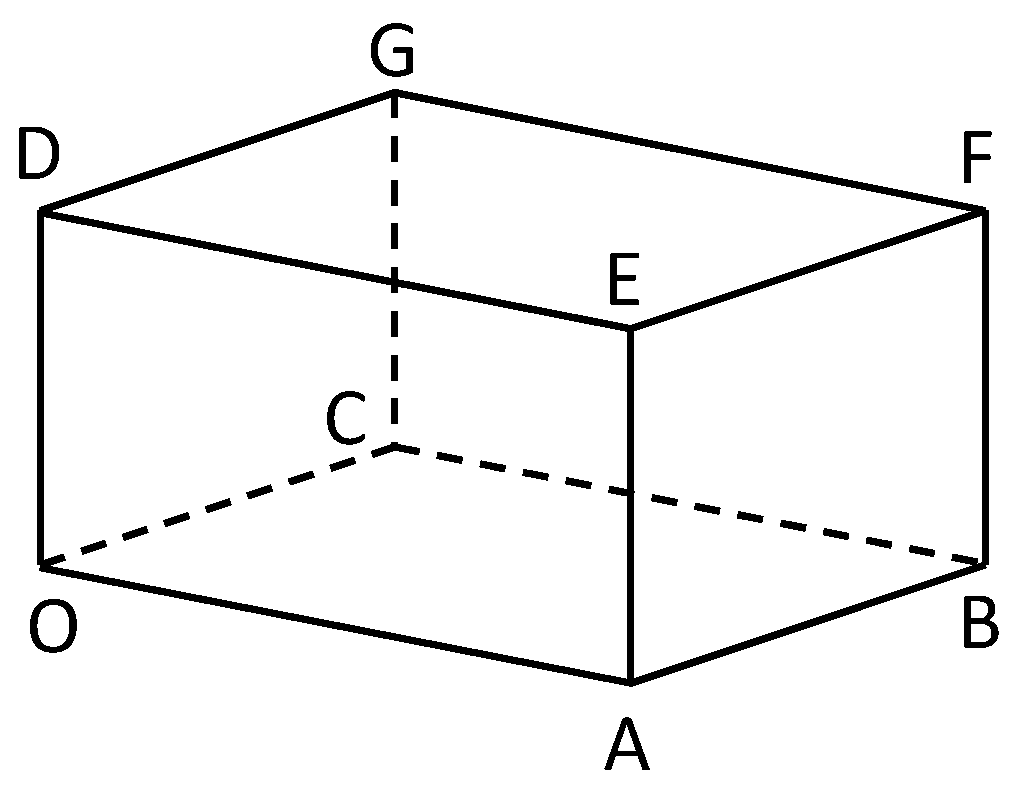
\includegraphics{img/vector_tyokuhotai.eps}
            }
        \end{center}
        \caption{直方体}
        \label{fig:vector_tyokuhotai}
    \end{figure}

    ただ,いちいち始点と終点を明示して表現するタイプのベクトルは書くのが面倒だ.加えて,1つのベクトルに対して複数の表現が存在するのは数学的にあまり好ましくはない.ここで3つのベクトルを代表として次のようにおく.
    \[
    \overrightarrow{\mathrm{OA}}=\vec{a},\mmm\overrightarrow{\mathrm{OC}}=\vec{c},
    \mmm \overrightarrow{\mathrm{OD}}=\vec{d}
    \]
    このようにすると
    \[
    \overrightarrow{\mathrm{OF}}=\vec{a}+\vec{c}+\vec{d}
    \]
    となる.ほかにも点Oからのベクトルに限り,$\vec{a},\vec{c},\vec{d}$を用いて簡潔に表現することができる.図形の中に1つ基準となる点を用意し,そこからの数個のベクトルによって図形上の任意の点を表現する方法はよく使われるので覚えておきたい.

    このような,"定点"を用意してベクトルを簡潔に表す,という発想が位置ベクトルにつながる.


    \section{位置ベクトル}
    算術的な計算のとき,$\vec{a},\vec{b}$はあくまで大きさと向きを備えた記号として扱ってきた.しかし,平面の図形となると始点と終点のほうが際立って扱われる.このことを前提に話を進めよう.

    \subsection{始点と終点\label{sub_sitenshuten}}
    先にも述べたようにベクトル入門におけるベクトルはあくまでベクトル量という意味でしかなかった.しかし,図形の問題におけるベクトルは始点と終点をつないだ有向線分という側面が強く現れる.
    始点と終点という意識が最も顕著に表れるのは$\overrightarrow{\mathrm{AB}},\overrightarrow{\mathrm{CD}}$といった始点と終点をそのまま書いてしまう書き方だ.

    このように図形におけるベクトルは始点と終点の2つで決定される.
    % 計算自体はベクトル入門で扱った方法でよい.

    \subsection{始点の共有\label{sub_sitenkyoyu}}
    直交座標を考えると,その座標というのはすべて原点からとってある.当たり前のことではあるが何か物の位置を定めるには,その基準となる定点が必要になるだろう.これをベクトルで考えてみる.

    図\ref{fig:vector_siten_kyoyu}のように定点Oから各点に有向線分を伸ばす.それらは\vecrm{OA} ,\vecrm{OB} などと表現される.このように必ず始点が一致しているベクトルを考えると,その始点をわざわざ書くことに一体どれほどの意味があるだろうか.これは必要ないと言っていいだろう.

    %
    \begin{figure}[htbp]
        \begin{center}
            \resizebox{!}{4cm}{
            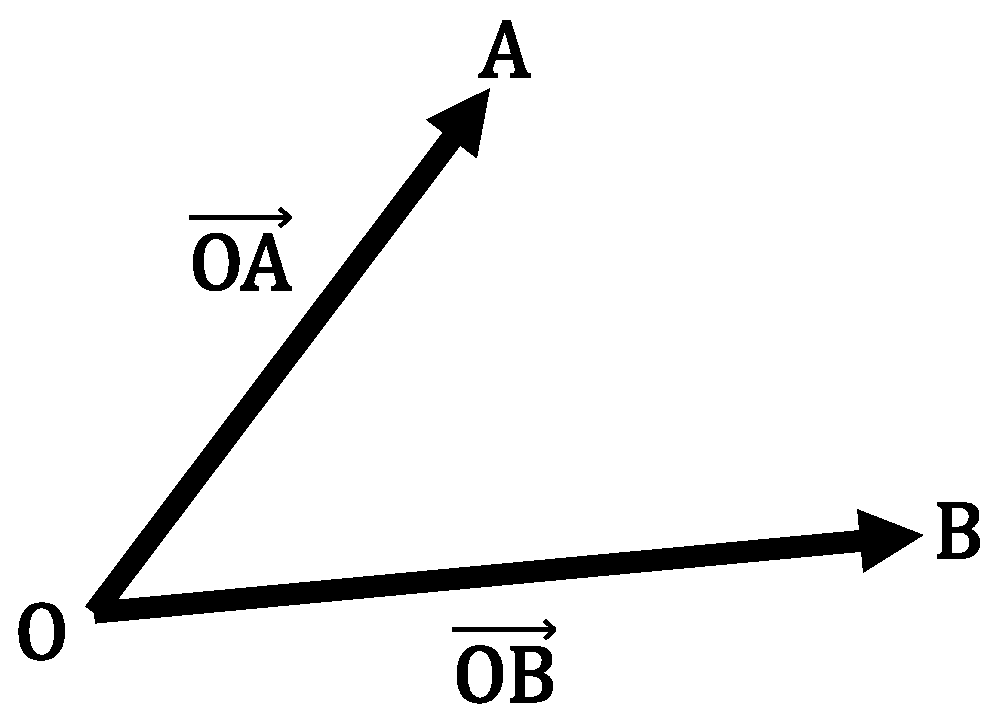
\includegraphics{img/vector_siten_kyoyu.eps}
            }
        \end{center}
        \caption{始点を共有した2ベクトル}
        \label{fig:vector_siten_kyoyu}
    \end{figure}

    このように始点を共有させるという条件のもと,さまざまな点へのベクトルを考えると,
    それは終点のみに注目している状態だということができる.

    \subsection{位置ベクトル}
    図\ref{fig:vector_hukusu_ten}のように空間に点がいくつかある状態を考える.
    %
    \begin{figure}[htbp]
        \begin{center}
            \resizebox{!}{3cm}{
            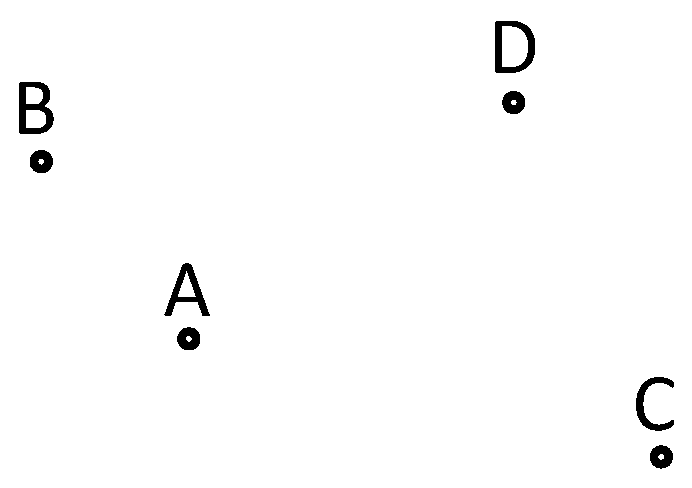
\includegraphics{img/vector_hukusu_ten.eps}
            }
        \end{center}
        \caption{空間上の複数の点}
        \label{fig:vector_hukusu_ten}
    \end{figure}

    このような状態でベクトルを作ると\vecrm{AB} のような2点の位置関係を表すベクトルができ,点Aや点Bだけに注目するようなベクトルは生まれない.
    ここでは\ref{sub_sitenkyoyu}節で扱った始点の共有の考え方を使う.
    % しかし,ここで前の小節で扱った始点の共有の考え方を使う.

    空間の中にどこでもいいから始点となる点Oを用意し,そこから\vecrm{OA} ,\vecrm{OB} などを考えてゆくとそれらのベクトルは終点であるAやBの位置のみを表すベクトルであるということができる.これを位置ベクトルといい,慣習として$\overrightarrow{\mathrm{OA}}=\vec{a}$のように小文字で書く.

    ここで理解を進めるため直交座標と位置ベクトルの対応をまとめる(表\ref{tab:Cartesian_vector}).

    \begin{table}[htbp]
        \caption{直交座標と位置ベクトル}
        \label{tab:Cartesian_vector}
        \begin{center}
            \begin{tabular}{|c|c|c|}\hline
                &直交座標&位置ベクトル\\ \hline
                基準点&原点&任意に定めた点O\\ \hline
                平面での2成分&x,y成分&大きさと向き\\ \hline
                空間での3成分&x,y,z成分&大きさと向き(2つ)\\ \hline
            \end{tabular}
        \end{center}
    \end{table}

    3次元空間で向きを決定するのに2つの成分が必要\footnote{星空を見上げるときに方角と高さの2つを気にすることから体感できるだろう.つまり,3次元空間で方向を決定しようと思うと2つの要素が必要になる.}だ.

    \subsection{位置ベクトルの理解}
    \ref{sub_sitenshuten}節では,図形の問題を扱う上でのベクトルは始点と終点を結ぶ有向線分の側面が大きいと述べた.しかし,表\ref{tab:Cartesian_vector}に示した位置ベクトルの性質は大きさと向きで決定するベクトル入門で大きく扱ったタイプのベクトルだ.これは始点を考えることがなくなったことが理由だ.そして,このことから位置ベクトルを1度導入したら,計算はベクトル入門におけるものをそのまま使えばよいことがわかる.

    また,大きさと向きで決定するタイプのベクトルはその中身\footnote{成分表示したときの内容.}が最後まで分からないことがほとんどだ\footnote{どの方向に向いていて,どれほどの大きさかはわからないまま問題が解けても良い.}.これは当然のことなので抵抗を感じないようにしてほしい.

    \section{位置ベクトルの利用}
    位置ベクトルの基本的な利用法を扱う.
    % 位置ベクトルの基本的な利用法を示す.理解を助けるため1次元座標との対応を考える.

    \subsection{点同士のベクトル}
    2点A(\veca),B(\vecb)を考える.AからBへのベクトルを\vecrm{AB}とする.これを位置ベクトルで表現すると,
    \[
    \overrightarrow{\mathrm{AB}} =\vec{b}-\vec{a}
    \]
   となる.位置ベクトルが始点を共有しているベクトルであることとベクトルの引き算を利用しているのだ.図\ref{fig:vector_iti_tendosi}がその参考になる.
   %
   \begin{figure}[htbp]
       \begin{center}
           \resizebox{!}{3cm}{
           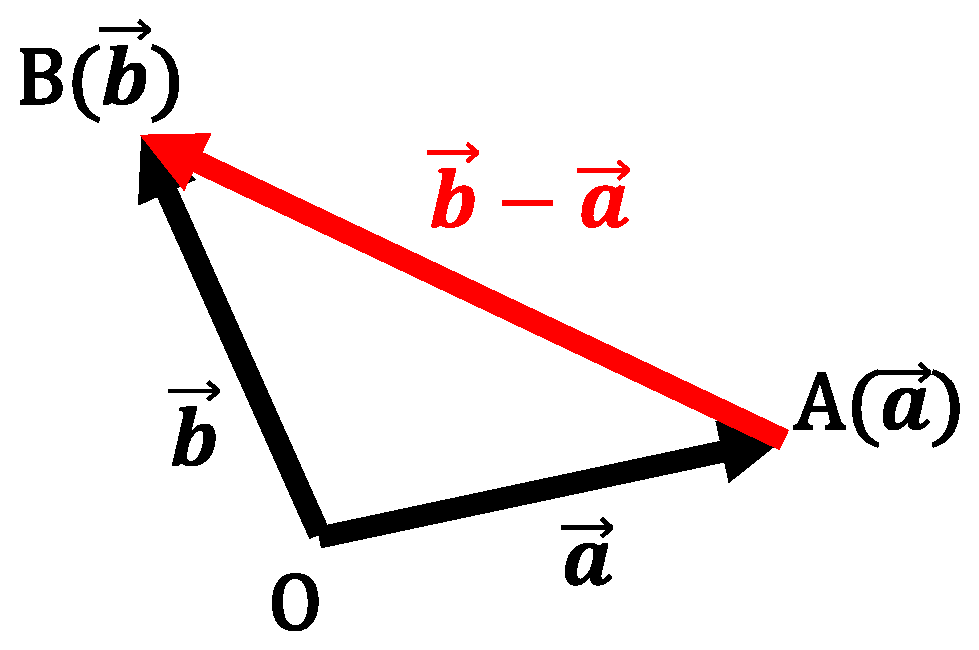
\includegraphics{img/vector_iti_tendosi.eps}
           }
       \end{center}
       \caption{2点間のベクトル}
       \label{fig:vector_iti_tendosi}
   \end{figure}

   \subsection{直線上の点\label{sub_tyokusen_ten}}
   直線AB上の点Pを表したい.例えば点P(\vecins{p})が線分ABをBの方向にABの$l$倍のばした位置にあるとする.直前の内容から$\overrightarrow{\mathrm{AB}} =\vec{b}-\vec{a}$となっていて,条件より
   \[
   \overrightarrow{\mathrm{AP}}=l\overrightarrow{\mathrm{AB}}
   \]
   であることがわかる.あとは位置ベクトルを代入し
   \begin{eqnarray*}
       \vec{p}-\vec{a}&=& l(\vec{b}-\vec{a})\\
       \therefore \vec{p}&=&(1-l)\vec{a}+l\vec{b}
   \end{eqnarray*}
   という結果を得る.係数の和が必ず1となることは頭の隅に置いておこう.


    \subsection{内分点}
    2点A(\veca),B(\vecb)を考える.この2点を$m:n$に内分する点P(\vecins{p})を考える.
    図\ref{fig:vector_iti_naibunten}のような状態だ.
    \vecins{p}は\veca と\vecrm{AB}を$m/(m+n)$倍との和といえよう.
    次のように計算される.

    \begin{eqnarray*}
        \vec{p}&=&\vec{a} +\frac{m}{m+n}\overrightarrow{\mathrm{AB}}\\
        &=& \vec{a}+\frac{m}{m+n}(\vec{b}-\vec{a})\\
        &=& \frac{n\vec{a}+m\vec{b}}{m+n}
    \end{eqnarray*}

    \begin{figure}[htbp]
        \begin{center}
            \resizebox{!}{3cm}{
            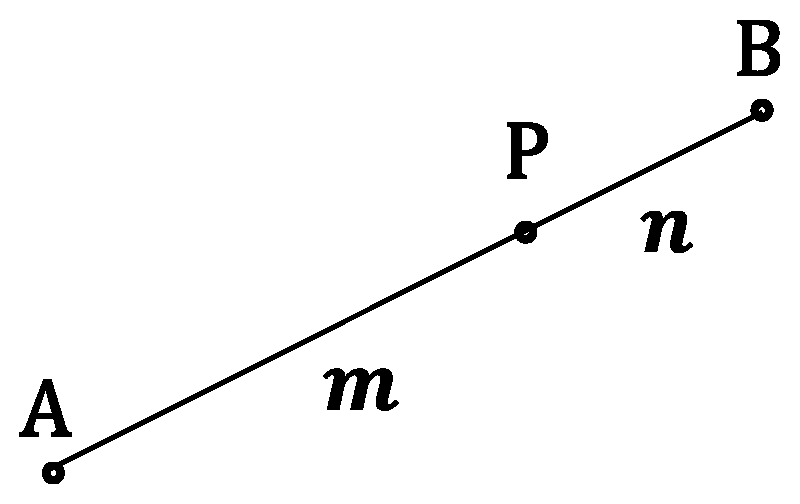
\includegraphics{img/vector_iti_naibunten.eps}
            }
        \end{center}
        \caption{内分点}
        \label{fig:vector_iti_naibunten}
    \end{figure}

    2点A(\veca),B(\vecb)を$m:n$に内分する点P(\vecins{p})が式(\ref{eq:naibunten_kosiki})と表されることを内分点公式という.
    \begin{equation}
        \vec{p}= \frac{n\vec{a}+m\vec{b}}{m+n}
        \label{eq:naibunten_kosiki}
    \end{equation}



    さらに,
    \[
    \frac{n\vec{a}+m\vec{b}}{m+n} =  \frac{n}{m+n}\vec{a} +\frac{m}{m+n}\vec{b}
    \]
    という関係から,係数の和が1となることがすぐにわかる.


    \subsection{外分点}
    2点A(\veca),B(\vecb)を考える.この2点を$m:n$に外分する点Pを考える.$m>n$であれば図\ref{fig:vector_iti_gaibunten1}のように,$m<n$であれば図\ref{fig:vector_iti_gaibunten2}のようになる.
    %
    \begin{figure}[htbp]
        \begin{center}
            \begin{tabular}{c}

                \begin{minipage}{0.45\hsize}
                    \begin{center}
                        \resizebox{!}{3cm}{
                        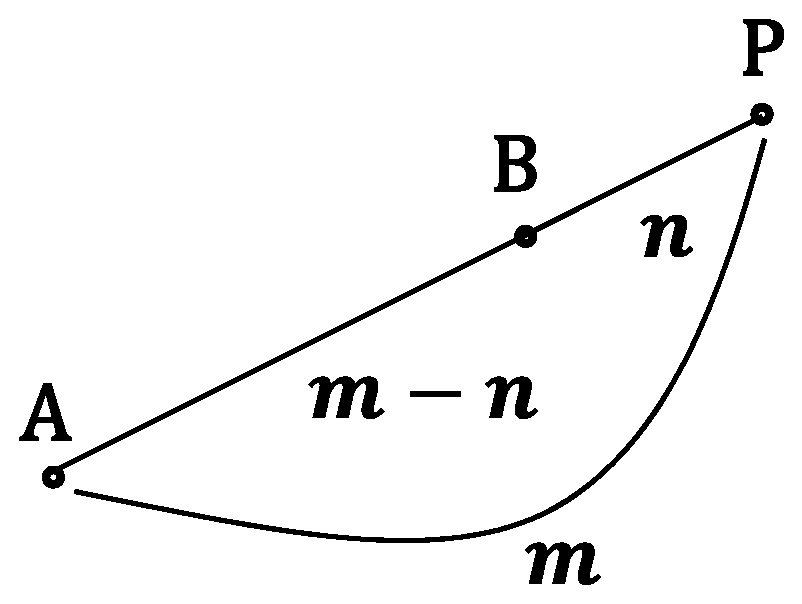
\includegraphics{img/vector_iti_gaibunten1.eps}
                        }
                    \end{center}
                    \caption{\mathins{m>n}}
                    \label{fig:vector_iti_gaibunten1}
                \end{minipage}

                \begin{minipage}{0.45\hsize}
                    \begin{center}
                        \resizebox{!}{3cm}{
                        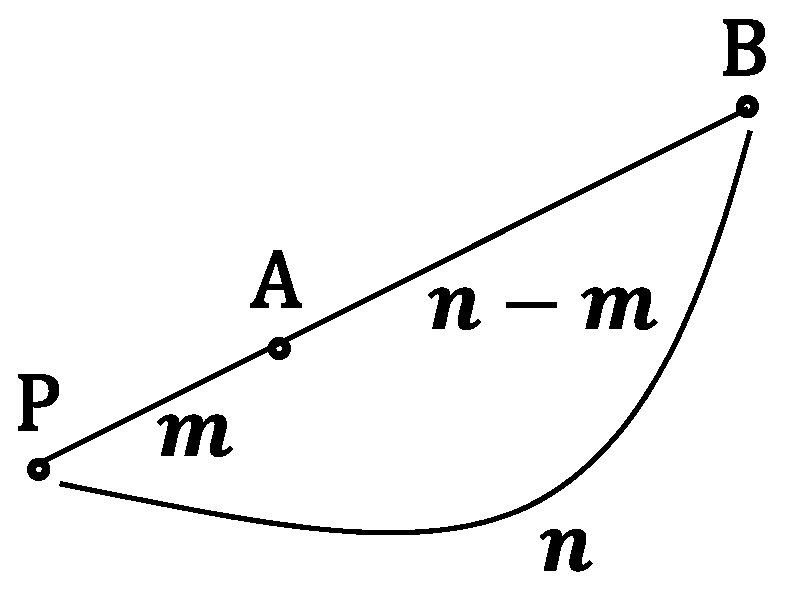
\includegraphics{img/vector_iti_gaibunten2.eps}
                        }
                    \end{center}
                    \caption{\mathins{m<n}}
                    \label{fig:vector_iti_gaibunten2}
                \end{minipage}

            \end{tabular}
        \end{center}
    \end{figure}

    これは$m,n$の大小で場合を分けて考える.$m>n$の場合,AとPに対して内分点公式を使い,Bの位置ベクトルを表す.$\mathrm{AB}:\mathrm{BP}=(m-n):n$より
    \begin{eqnarray*}
        \vec{b} &=& \frac{n\vec{a}+(m-n)\vec{p}}{(m-n)+n}\\
        &=& \frac{n}{m}\vec{a} +\frac{m-n}{m}\vec{p}\\
        \Leftrightarrow \vec{p}&=&\frac{-n\vec{a}+m\vec{b}}{m-n}
    \end{eqnarray*}
    と計算される.

    次に$m<n$の場合,PとBに対して内分点公式を使い,Aの位置ベクトルを表す.$\mathrm{PA}:\mathrm{AB}=m:(n-m)$より
    \begin{eqnarray*}
        \vec{a}&=& \frac{(n-m)\vec{p}+m\vec{b}}{m+(n-m)}\\
        &=& \frac{n-m}{n}\vec{p} +\frac{m}{n}\vec{b}\\
        \Leftrightarrow \vec{p}&=&\frac{n\vec{a}-m\vec{b}}{n-m}\\
        &=&\frac{-n\vec{a}+m\vec{b}}{m-n}
    \end{eqnarray*}
    と計算され,$m,n$の大小関係によらずに同じ結果を得ることができた.

    以上より2点A(\veca),B(\vecb)を$m:n$に外分する点P(\vecins{p})が式(\ref{eq:gaibunten_kosiki})であらわされることを外分点公式という.これはA,Bを$m:(-n)$に内分していると解釈することもできる.
    \begin{equation}
        \vec{p}=\frac{-n\vec{a}+m\vec{b}}{m-n}
        \label{eq:gaibunten_kosiki}
    \end{equation}

    ここでも係数を取り出して考える.
    \[
    \vec{p} = \frac{-n\vec{a}}{m-n}+\frac{m\vec{b}}{m-n}
    \]

    足したら1となるのはここでも同じだ.
    既に\ref{sub_tyokusen_ten}節で一直線上にある点の話でこのことは説明している.
    位置ベクトル\mathins{\vec{a},\vec{b}}を含む直線上の点の位置を2つのベクトルであらわすと係数の和が1となるのだ.ここまでくどいのは問題を解く上で重要な要素となるからである.また,係数がともに正であれば内分点,負のものが含まれれば外分点となることもあわせて覚えよう.

    \subsection{三角形の重心}
    ここまでの位置ベクトルの基本的な利用をおさらいする.


    $\bigtriangleup \mathrm{ABC}$の重心を$\mathrm{G}(\vec{g})$とする.各頂点を$\mathrm{A}(\vec{a}),\mathrm{B}(\vec{b}),\mathrm{C}(\vec{c})$とすると重心の位置ベクトルは
    \[
    \vec{g}=\frac{\vec{a}+\vec{b}+\vec{c}}{3}
    \]
    となる.

    証明の前に,数Aを思い出そう.三角形の重心とは各頂点からの中線の交点と定義されている.さらに,重心は中線を2:1に内分している(図\ref{fig:vector_sankaku_jusin}).

    \begin{figure}[htbp]
        \begin{center}
            \resizebox{!}{3cm}{
            \includegraphics{img/vector_sankaku_jusin.eps}
            }
        \end{center}
        \caption{三角形の重心}
        \label{fig:vector_sankaku_jusin}
    \end{figure}
    %三角形の重心

    では証明に入る.点Aから線分BCの中点へのベクトルを考える.
    \[
    \frac{1}{2}(\vec{b}+\vec{c})-\vec{a}
    \]
    このベクトルを$2/3$倍することで点Aから重心へのベクトルを計算することができる.
    \[
    \overrightarrow{\mathrm{AG}}=-\frac{2}{3}\vec{a}+\frac{1}{3}\vec{b}+\frac{1}{3}\vec{c}
    \]
    となる.最後に$\overrightarrow{\mathrm{AG}}=\vec{g}-\vec{a}$を代入して式を変形することで
    \[
    \vec{g}=\frac{\vec{a}+\vec{b}+\vec{c}}{3}
    \]
    を得る.



    \section{平面図形とベクトル}
    基本的な使い方に加え,より実践的なベクトルの利用を平面図形において扱う.漠然とした話のみをする.具体的には問題を解く際に扱う.そのため読み飛ばしてもらって構わない.



    \subsection{一直線上にある3点(1)}
    点A,B,Cが一直線上にあるとはどういうことか.ベクトル入門の内容から考えるに
    \[
    \overrightarrow{\mathrm{AB}}=k\overrightarrow{\mathrm{AC}}
    \]
    を満たす実数$k$が存在することを証明すればよいだろう.\\

    ここで話はそれるが,高校数学において存在を証明する手段と証明できるものを挙げる.
    \begin{description}
        \item[2次方程式の判別式] 2次方程式に実数の解が存在するのか.また,いくつ存在するのかを明らかにする.
        \item[中間値の定理] 連続な関数であれば,端点の値の間にある値は必ず存在することを証明する.
        \item[平均値の定理] 連続な関数であれば,端の2点で計算される傾きと同じ傾きになる点が少なくとも1つ存在することを証明する.
    \end{description}
    このように高校数学では"存在の証明"の方法が3つしかない.そのほかにも存在だけを考えればよいことは少なくないが,存在だけの言及はできなものと考えたほうが良い.

    では,3点が一直線上にあることを示す$k$の存在はどのように証明するのか.これに対する答えは,$k$の値を明らかにすることだ.値を持つということが存在することの十分条件となる.高度な問題に関しては値を計算すればよいところを,"存在を証明せよ"とわざと誤導することがある.先に挙げた3つの存在証明の性質を理解した上で,場合によっては値を求めることで存在を証明しよう.

    \subsection{一直線上にある3点(2)}
    一直線上にある3点という話を位置ベクトルにも近い話でもう一度扱う.
    図のように定点Oからのベクトル\mathins{\overrightarrow{OA},\overrightarrow{OB}}をとる.これらは一次独立とし,その直線上に点Pがあるとする.
    \begin{figure}[htbp]\centering
        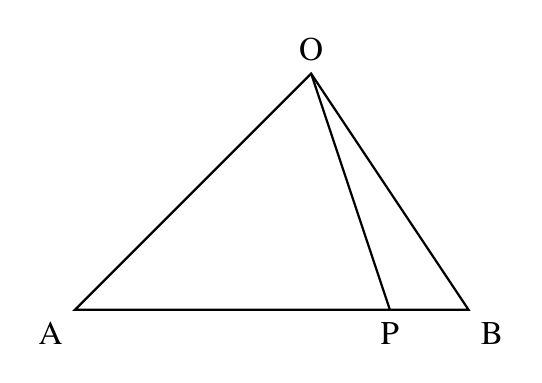
\begin{tikzpicture}\large
            \coordinate (o) at (0,0);
            \coordinate (a) at (-3,-3);
            \coordinate (b) at (2,-3);
            \draw[thick](o)node[above]{O}--(a)node[below left]{A}--(b)node[below right]{B}--cycle;

            \coordinate (p) at (1,-3);
            \draw[thick](o)--(p)node[below]{P};

        \end{tikzpicture}
        \caption{一直線上にある定点}
        \label{tikz:ittyokusen_teiten}
    \end{figure}

    このようにすると,先の話を利用することで
    \[
    \overrightarrow{AB} =k \overrightarrow{AP}\quad{k:\text{実数}}
    \]
    と分かる.これを定点Oからの位置ベクトルとする.
    \begin{align*}
        \overrightarrow{AB} &=k \overrightarrow{AP}\\
        \Leftrightarrow (\overrightarrow{OB}-\overrightarrow{OA})
        &= k(\overrightarrow{OP}-\overrightarrow{OA})\\
        \therefore \overrightarrow{OP}
        &= (1-k)\overrightarrow{OA}+k\overrightarrow{OB}
    \end{align*}

    これは点Pが線分ABを\mathins{k:1-k}に内分したときの内分点公式の結果にも見える.しかし,大事なのは\mathins{k}が実数であるところだ.そのため\mathins{k}は様々な値をとる.例えば\mathins{k}が負の値であるときは点Pは点Aより左側にあり,\mathins{k}が1より大きな値では点Pは点Bの右側にある.つまり,\mathins{k}の値によってPは直線AB上のいかなる点も取ることができる.

    無数のPの位置に対して共通するのは\mathins{\overrightarrow{OA},\overrightarrow{OB}}の係数の値が常に1で一定である点だ.これは逆も成立する話で次のようにまとめられる.
    \begin{itembox}[l]{一直線上の3点の位置ベクトル}
        一次独立なベクトル\mathins{\overrightarrow{OA},\overrightarrow{OB}}に対し,\mathins{\overrightarrow{OP}}が次のように表現されることと,A,B,Pが同一直線上にあることは同値である.
        \[
        \overrightarrow{OP}=s\overrightarrow{OA}+t\overrightarrow{OB},\qquad s+t=1
        \]
    \end{itembox}

    これは定点Oを省略して位置ベクトルでも同様のことが言える.3点が同一直線上にあるということは2つの表現の方法がある.



    \subsection{1次独立}
    この語句は印象に残りやすいものなので,その意味を含めてすでに理解しているかもしれない.空間図形の節でも扱うので読み飛ばしてもらって構わない.

    まずは1次独立とはどういうものなのかを示す.
    \begin{screen}
        ある平面上に存在する\vecins{0} ではない2つのベクトル\veca ,\vecb があるとき,この2つのベクトルが平行でないならば,これらは1次独立であるという.

        さらに,ある平面上で1次独立な関係である2つのベクトル\vecx ,\vecy をとったならば,その平面上の任意のベクトル\vecz は,ある実数$a,b$をもって
        \[
        \vec{z}=a\vec{x}+b\vec{y}
        \]
        と表される.そしてこの実数の組$(a,b)$は,ただ1つに定まる.
    \end{screen}
    これはベクトル入門で扱ったベクトルの分解に関係する話だ.ベクトル入門では分解する先の2つのベクトルはすでに与えられていた.その2つのベクトルとはこの1次独立の関係であるものが選ばれているのだ.

    1次独立で最も重要なのはベクトルを分解した後の係数の組\mathins{a,b} がただ1つに定まるということだ.これを一意性といって,問題を解く上で極めて強力な条件を与える.具体的な使い方は問題で扱う.

    \subsection{斜交座標}
    直交座標というのはベクトルから理解すると,(1,0),(0,1)の2つの単位ベクトルの線形和\footnote{実数をかけた上で,和をとることを線形和という.}によって位置を決定している座標ということになる.
    \[
    (3,-4)=3(1,0)-4(0,1)
    \]
    これは,2つの単位ベクトルが1次独立の関係にあることが重要だ.このため,どのような座標上の点も表すことができる.

    先の小節では平面における1次独立を扱った.1次独立には単位ベクトルである必要も直交している必要もない.つまり,図\ref{fig:vector_shako_zahyo}のような軸をとっても平面上のすべての点を表すことができるのだ.これを斜交座標という.
    %斜交座標の図
    \begin{figure}[htbp]
        \begin{center}
            \resizebox{!}{5cm}{
            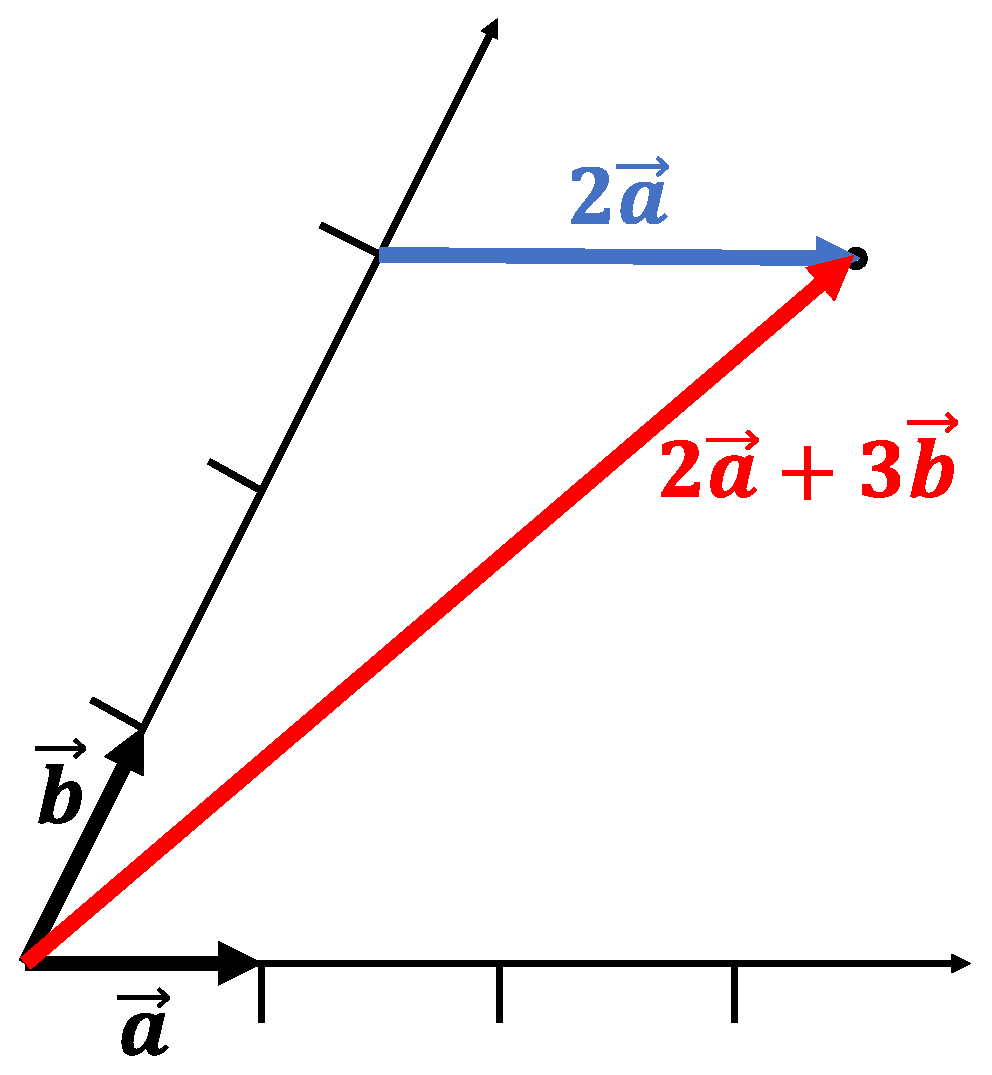
\includegraphics{img/vector_shako_zahyo.eps}
            }
        \end{center}
        \caption{斜交座標}
        \label{fig:vector_shako_zahyo}
    \end{figure}

    図\ref{fig:vector_shako_zahyo}の例では斜交座標における座標は(2,3)となる.

    ベクトル入門では\mathins{(1,2)}のようなベクトルはお約束となるベクトルの係数をとってきた表現であると説明した.斜交座標ではこのお約束のベクトルが1次独立なベクトルの組に置き換わっているのだ.具体的な用法はのちの問題で扱う.



    \section{空間図形とベクトル}

    \subsection{ベクトルの利用価値}
    空間図形に対してベクトルを利用する前に,ベクトルの利用価値について述べたい.ベクトルの本質とは"大きさ"と"向き"を矢印のついた記号に押し込んでしまえば,ベクトル入門で扱った計算法を守るだけで正しい議論が可能であるという点だ.そして,この性質は空間図形において顕著に表れる.位置ベクトルの節において,表\ref{tab:Cartesian_vector}を示した.ここには3次元空間での向きは2つの成分で決定する旨を説明している.つまり,3次元空間を扱うならば本来3つの成分\footnote{大きさ,向き1,向き2の3つ.}を相手にする必要があるのだ.しかし,ベクトルを導入するとその成分は"大きさ","向き"と縮小される.さらに,ベクトル入門の計算則を守れば,矢印のついた記号1つを相手にすればよいことになる.

    これは,ベクトルのルールを守ることを前提に次元数を小さくしているということだ.もちろんベクトルが万能というわけでもない.ベクトルの計算体系は図\ref{fig:vector_sanjutukeisan_taikei}に示した通りであるので,図形的な条件や仮定がない場合は計算自体ができないことも考えれる.2次試験で解法をベクトルに求めるときには注意が必要だ.

    \subsection{一直線上にある3点}
    これは平面での話と同じだ.ただ,問題として出題されるのは空間図形での話が多い.


    \subsection{同じ平面上にあるベクトル}
    3次元空間で1つの平面を決定するときは条件のいずれか1つを満たすことが必要だ.
    \begin{itemize}
        \item 3つの定点がある
        \item 1本の直線と1つの定点がある
        \item 平行な2直線がある
    \end{itemize}
    このような条件に該当するとき平面は決定する.では,始点を共有する2つ異なるのベクトル\veca ,\vecb を考える.ただし,これらはともに\vecins{0} ではない.共有された始点1つと異なる終点2つの3点によって平面が決定する(図\ref{fig:vector_hemen_itijidokusitu}).この2つのベクトルは1次独立な関係になっている.
    %平面とベクトル
    \begin{figure}[htbp]
        \begin{center}
            \resizebox{!}{3cm}{
            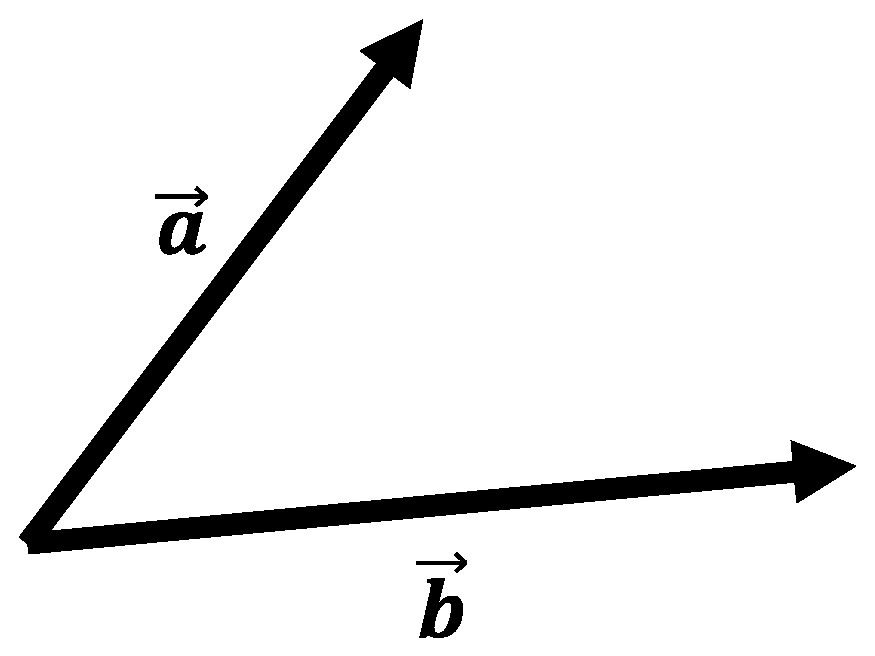
\includegraphics{img/vector_hemen_itijidokusitu.eps}
            }
        \end{center}
        \caption{1次独立}
        \label{fig:vector_hemen_itijidokusitu}
    \end{figure}

    1次独立なベクトル\veca ,\vecb で決定された平面上にベクトル\vecins{c} をとると,いかなる\vecins{c} に対しても
    \[
    \vec{c}=s\vec{a}+t\vec{b}
    \]
    を満たす実数の組$s,t$が存在し,その組はただ1つに定まる.

    あるベクトル\vecins{d} が
    \[
    \vec{d}=k\vec{a}+l\vec{b}\mmm (k,l\in \mathbb{R})
    \]
    であるならば,\vecins{d}は\veca,\vecb の決定する平面上に存在する.

    これは,平面図形での話の続きになる内容だ.結論としては,平面を決定することができる2つのベクトル\footnote{大きさが0ではない,異なる2つのベクトル.}の線形和であらわされるベクトルは,元の2つのベクトルで決定される平面上のベクトルであるといことだ.

    4点が同じ平面に存在するかどうかは,4つのうちの1つを始点とした3つのベクトルで上の関係が成立するのかを確認すればいい.


    \subsection{空間での1次独立}
    3次元空間での1次独立は平面のものとは少し異なる.
    \begin{screen}
        空間に\veczero ではない3つのベクトル\veca,\vecb,\vecins{c} をとる.\veca,\vecb が平行ではなく,
        \[
        \vec{c}=s\vec{a}+t\vec{b}
        \]
        を満たす実数の組\mathins{s,t}がないとき,これらのベクトルは1次独立であるという.

        空間上に1次独立なベクトル\veca,\vecb,\vecins{c} をとる.すると,空間上に存在するすべてのベクトル\vecins{p} は
        \[
        \vec{p}=s\vec{a}+t\vec{b}+u\vec{c}\mmm(s,t,u\in \mathbb{R})
        \]
        と表される.そして実数係数の組\mathins{(s,t,u)}は一意に定まる.
    \end{screen}
    かみ砕いて説明すると,空間における1次独立とは同じ平面に存在しない4つの点の関係を述べている.3点で1つの平面が決定するが,4つ目の点はその平面に存在していない.これは図\ref{fig:vector_tyokuhotai}における\veca,\vecins{c},\vecins{d} の関係だ.


    % \section{ベクトルと図形での問題}
    % \subsection{図形の性質をベクトルから確認}
    % \begin{itembox}[l]{問題}
    %     \begin{enumerate}
    %         \item 平行四辺形
    %         \item
    %         \item
    %         \item
    %         \item
    %         \item
    %         \item
    %     \end{enumerate}
    % \end{itembox}




\end{document}
